\section{Figures}
\label{app:figures}

Every figure below is drawn by \code{src/figures\_phase2.py} from the same CSV
tables the body's numbers come from, so a figure cannot disagree with a table.

\begin{figure}[htbp]
  \centering
  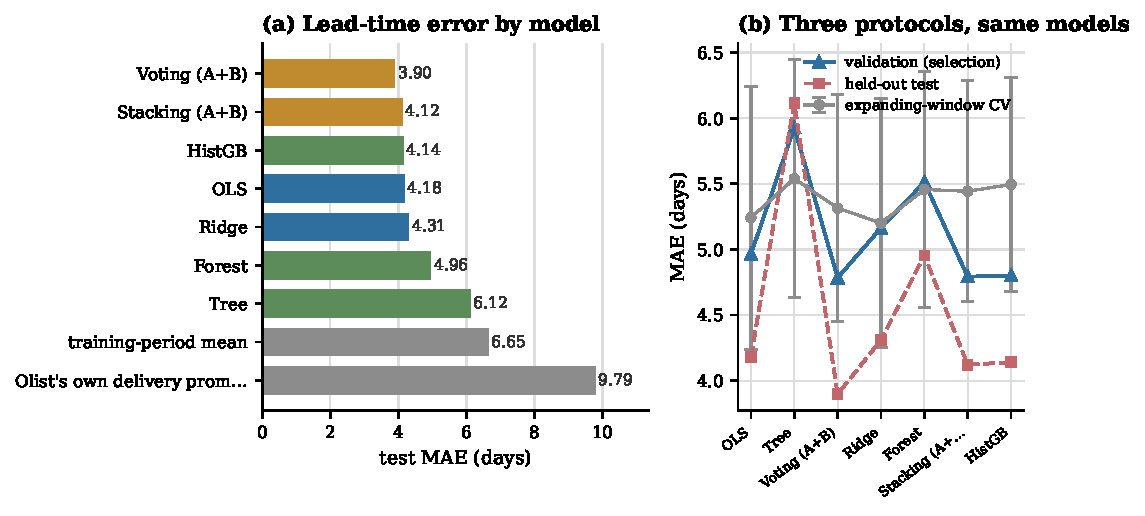
\includegraphics[width=\linewidth]{fig10_regression_ladder.pdf}
  \caption{Lead-time error by model, and the same models under three protocols.
  Panel (b) is the argument of Section~\ref{sec:cv}: expanding-window
  cross-validation does not order the candidates the way the validation period
  and the forward window --- which agree with each other --- do.}
  \label{fig:ladder}
\end{figure}

\begin{figure}[htbp]
  \centering
  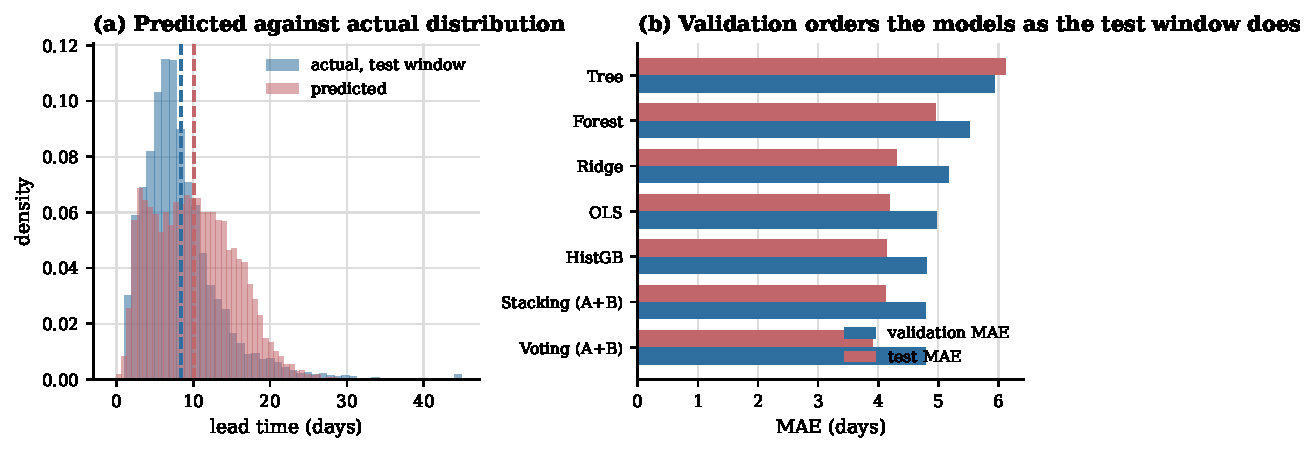
\includegraphics[width=\linewidth]{fig19_extrapolation.pdf}
  \caption{Why blending a linear model with a boosted one helps under drift. A
  tree cannot predict outside the range of the targets it was fitted on; lead
  times in the test window are systematically shorter than anything common in
  training. Panel (b) shows the validation period ordering the models as the test
  window does.}
  \label{fig:extrap}
\end{figure}

\begin{figure}[htbp]
  \centering
  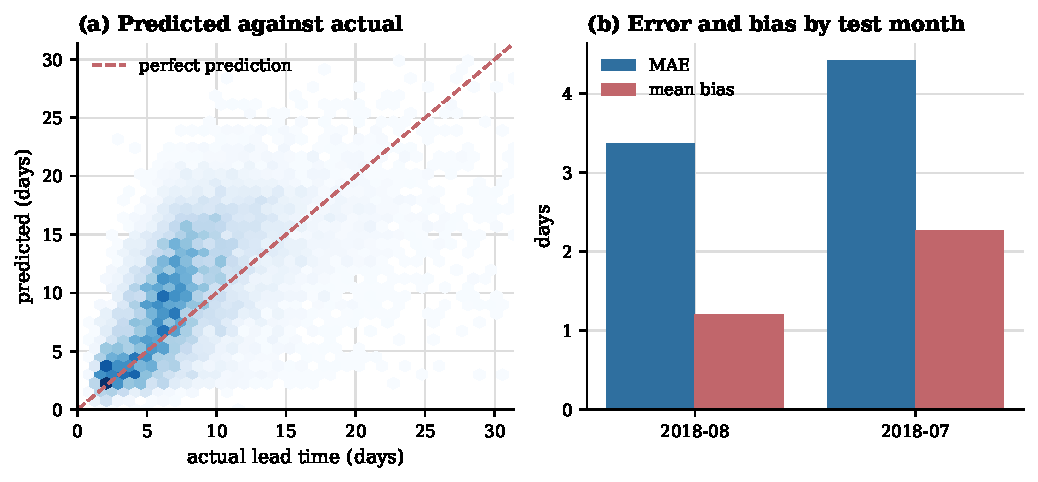
\includegraphics[width=\linewidth]{fig11_regression_residuals.pdf}
  \caption{Where the regression is wrong. The bias in panel (b) is positive in
  both test months: a model fitted on a slower past over-predicts how long a
  parcel will take.}
  \label{fig:resid}
\end{figure}

\begin{figure}[htbp]
  \centering
  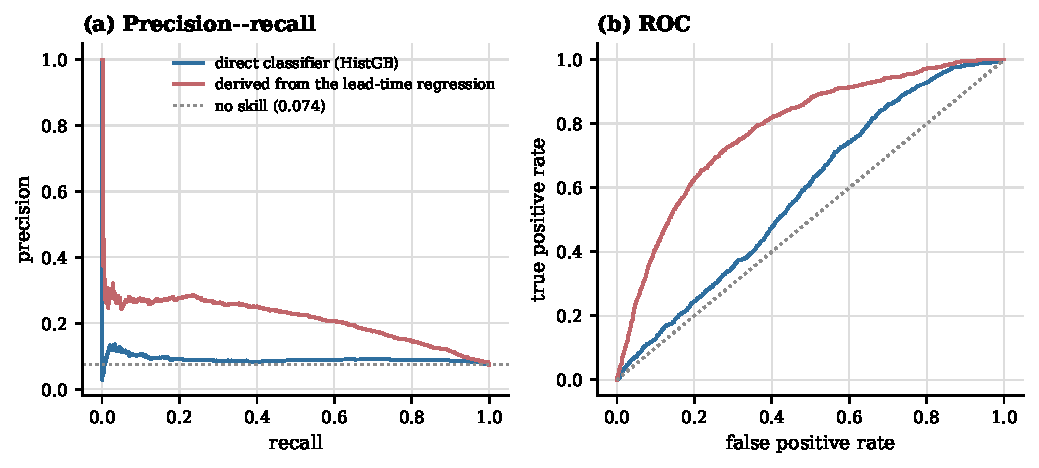
\includegraphics[width=\linewidth]{fig12_late_routes.pdf}
  \caption{Problem 1B. The flag derived from the lead-time regression against the
  best purpose-built classifier, on the forward test window.}
  \label{fig:routes}
\end{figure}

\begin{figure}[htbp]
  \centering
  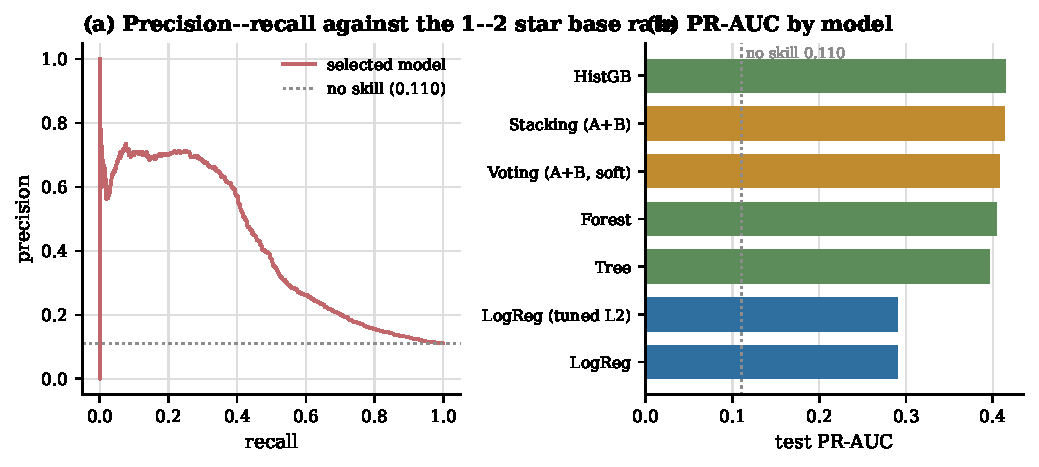
\includegraphics[width=\linewidth]{fig13_low_review.pdf}
  \caption{Problem 2 against its no-skill floor, and PR-AUC by model. Most of the
  achievable signal is already available from a single depth-limited tree.}
  \label{fig:lowreview}
\end{figure}

\begin{figure}[htbp]
  \centering
  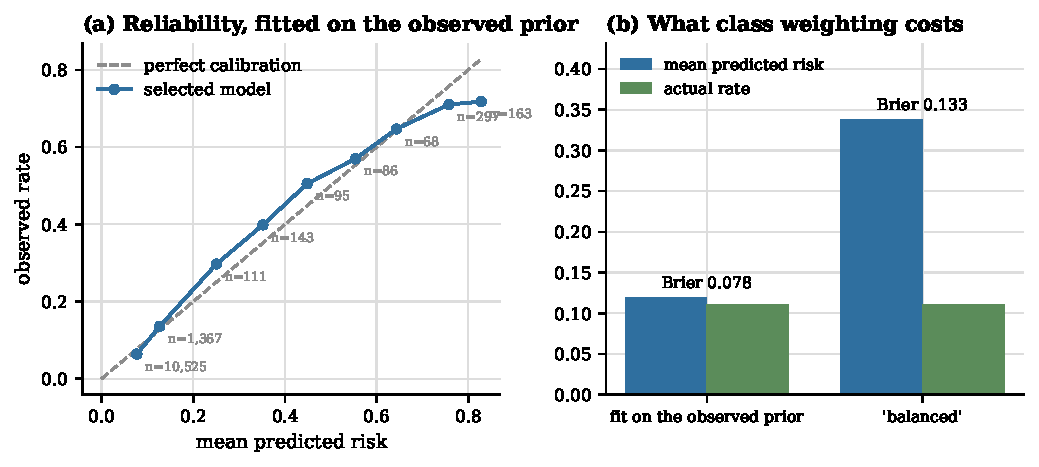
\includegraphics[width=\linewidth]{fig14_calibration.pdf}
  \caption{Calibration, and what class weighting costs. Weighting the loss leaves
  ranking unchanged and inflates mean predicted risk threefold against the actual
  rate.}
  \label{fig:calibration}
\end{figure}

\begin{figure}[htbp]
  \centering
  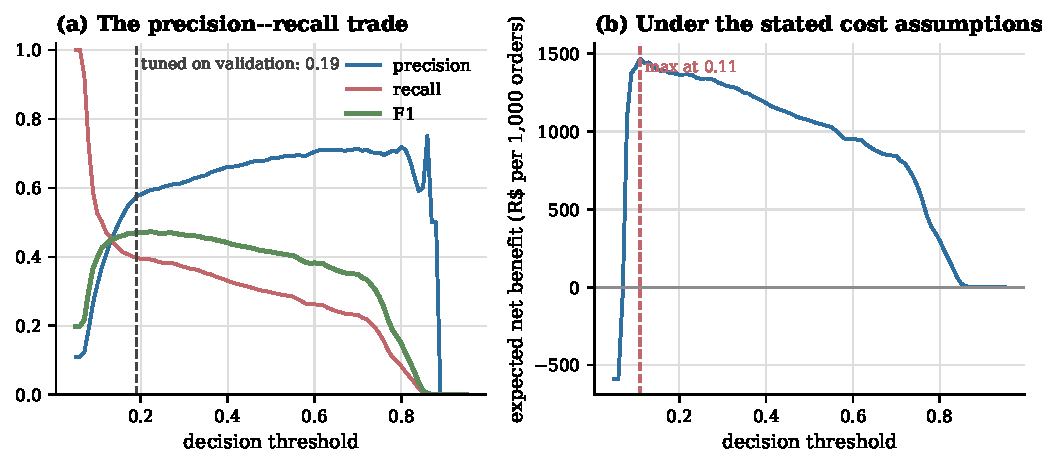
\includegraphics[width=\linewidth]{fig15_threshold_cost.pdf}
  \caption{Choosing the operating point for the review model, and what it is
  worth under the stated cost assumptions.}
  \label{fig:threshold}
\end{figure}

\begin{figure}[htbp]
  \centering
  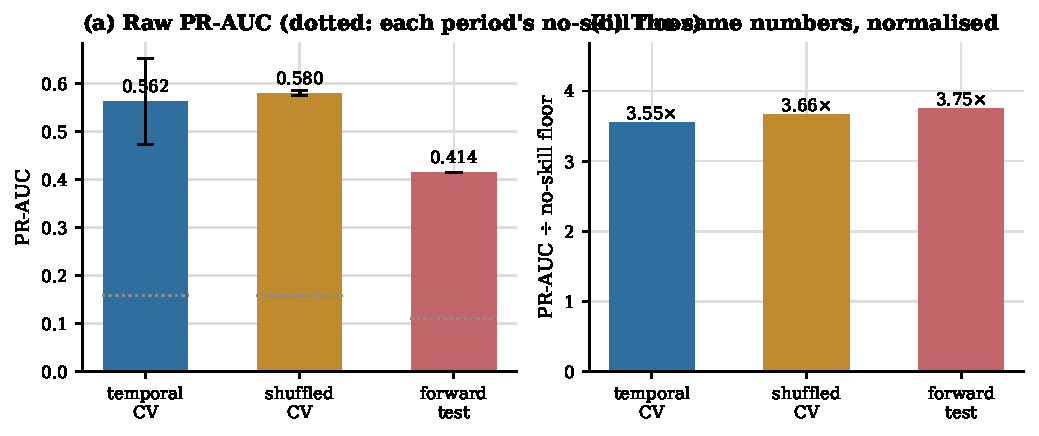
\includegraphics[width=\linewidth]{fig16_cv_protocol.pdf}
  \caption{One model, three protocols. Raw average precision disagrees across
  periods; divided by each period's no-skill floor the three agree to within 0.2
  of a multiple.}
  \label{fig:protocol}
\end{figure}

\begin{figure}[htbp]
  \centering
  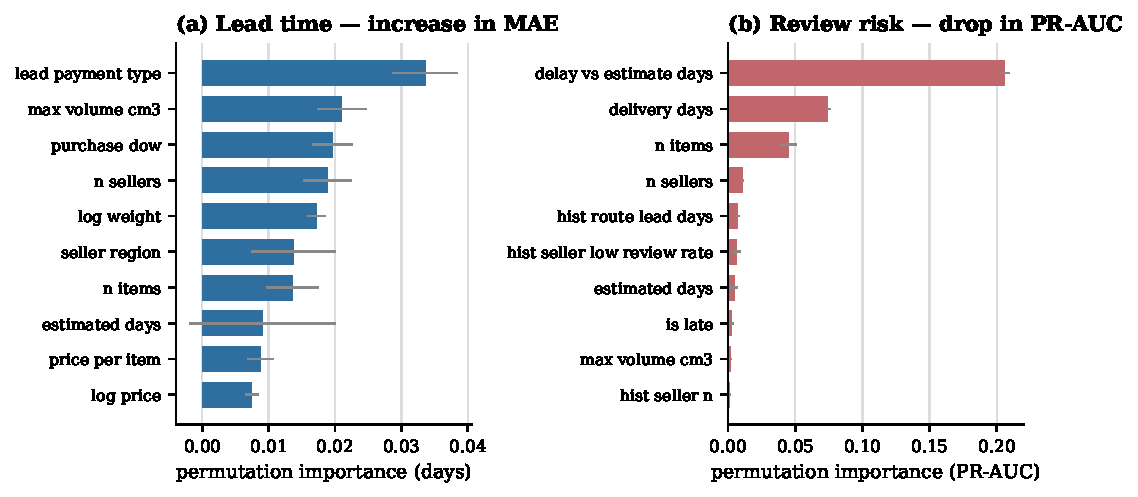
\includegraphics[width=\linewidth]{fig17_importance.pdf}
  \caption{Permutation importance on the test window. The review model rests on
  two features; the lead-time model on none in particular, which is a property of
  correlated predictors as much as of the model.}
  \label{fig:importance}
\end{figure}

\begin{figure}[htbp]
  \centering
  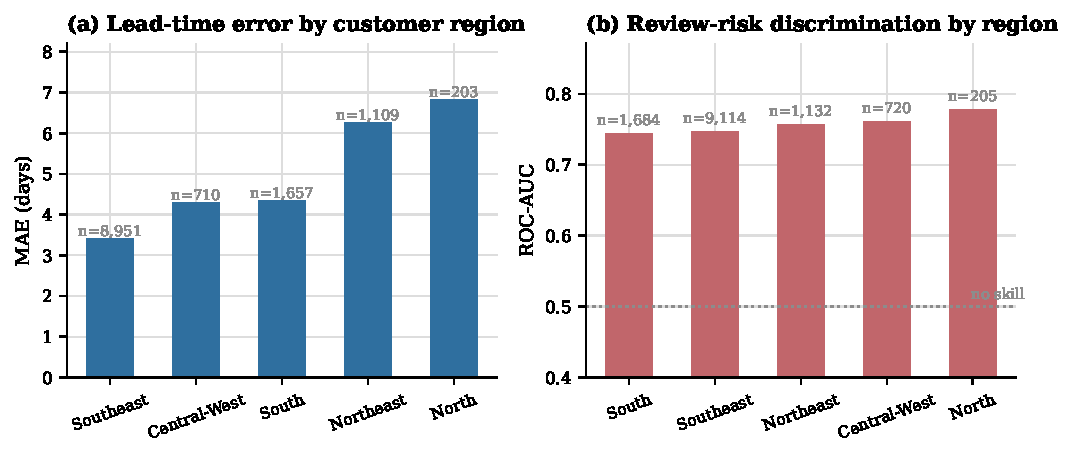
\includegraphics[width=\linewidth]{fig18_segments.pdf}
  \caption{Performance by customer region. The review model is stable across all
  five; the regression is not, and degrades exactly where deliveries are
  longest.}
  \label{fig:segments}
\end{figure}

\begin{figure}[htbp]
  \centering
  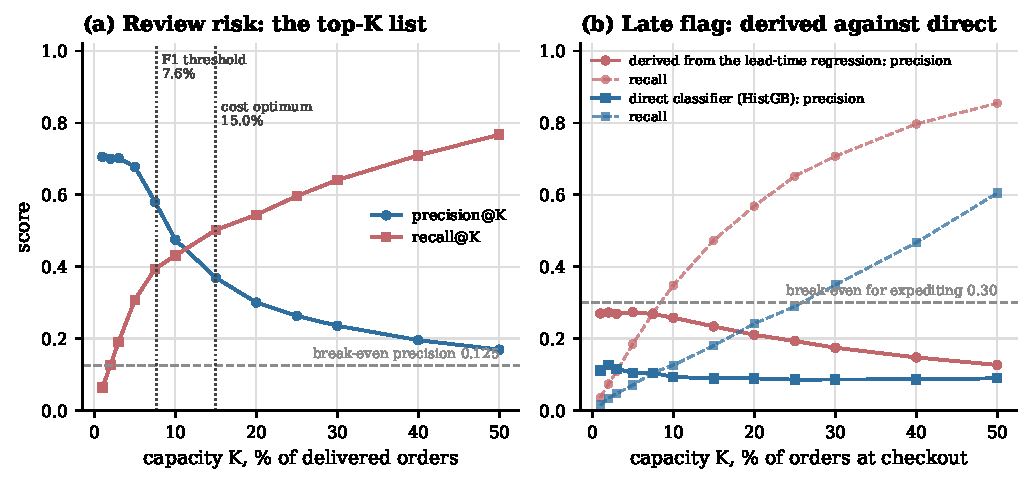
\includegraphics[width=\linewidth]{fig20_capacity.pdf}
  \caption{Precision and recall when only the top $K$ can be acted on
  (Section~\ref{sec:results-capacity}). (a) The review-risk list, with the
  report's two threshold operating points placed on the capacity axis; precision
  stays above the break-even at every capacity. (b) The late flag: the derived
  route beats the direct classifier at every $K$ and never reaches the
  break-even an expensive expedite would need.}
  \label{fig:capacity}
\end{figure}

\begin{figure}[htbp]
  \centering
  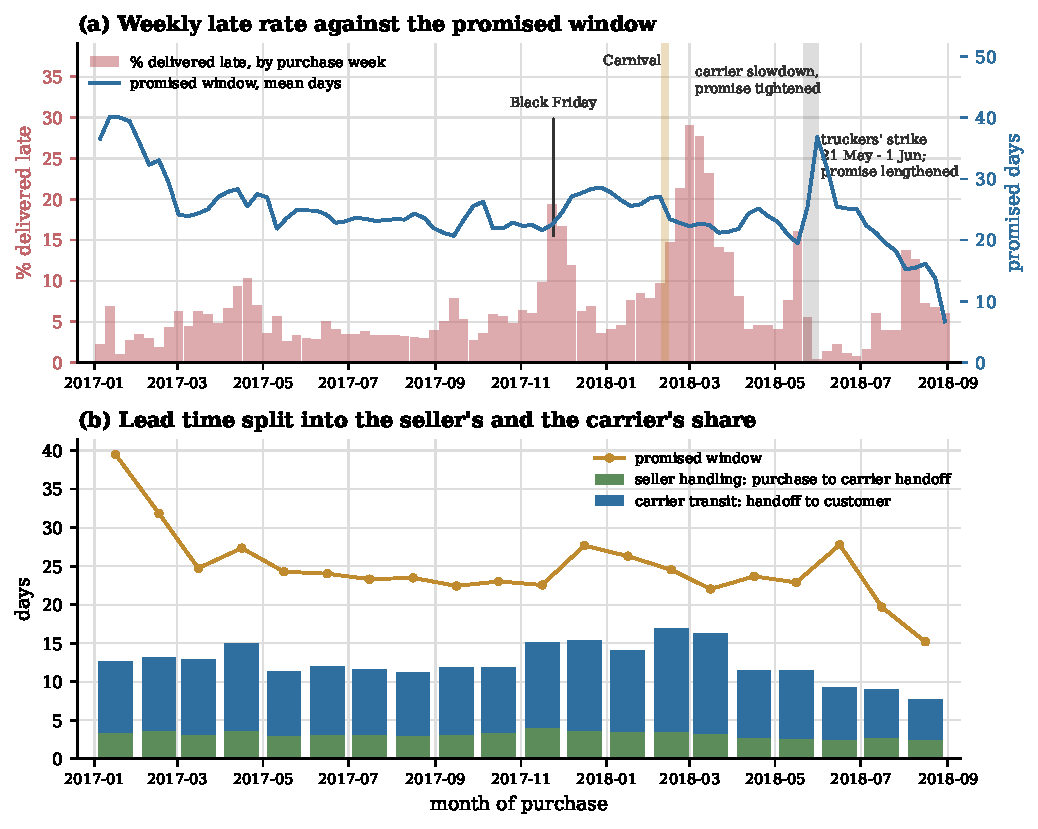
\includegraphics[width=\linewidth]{fig21_lateness_anatomy.pdf}
  \caption{Where the late deliveries came from (Appendix~\ref{app:lateness}).
  (a) Weekly late rate against the promised window: the February--March 2018
  peak coincides with a tightened promise, and the strike of 21 May--1 June 2018
  (shaded) hits the week promised before it, after which the promise is
  lengthened and the late rate collapses. (b) Lead time split at the carrier
  handoff: the peak is carrier transit, not seller handling.}
  \label{fig:lateness}
\end{figure}
